\documentclass{standalone}
\usepackage{tikz}
\usetikzlibrary{patterns, positioning}
\usepackage[sfdefault]{ClearSans} %% option 'sfdefault' activates Clear Sans as the default text font
\usepackage[T1]{fontenc}

\begin{document}
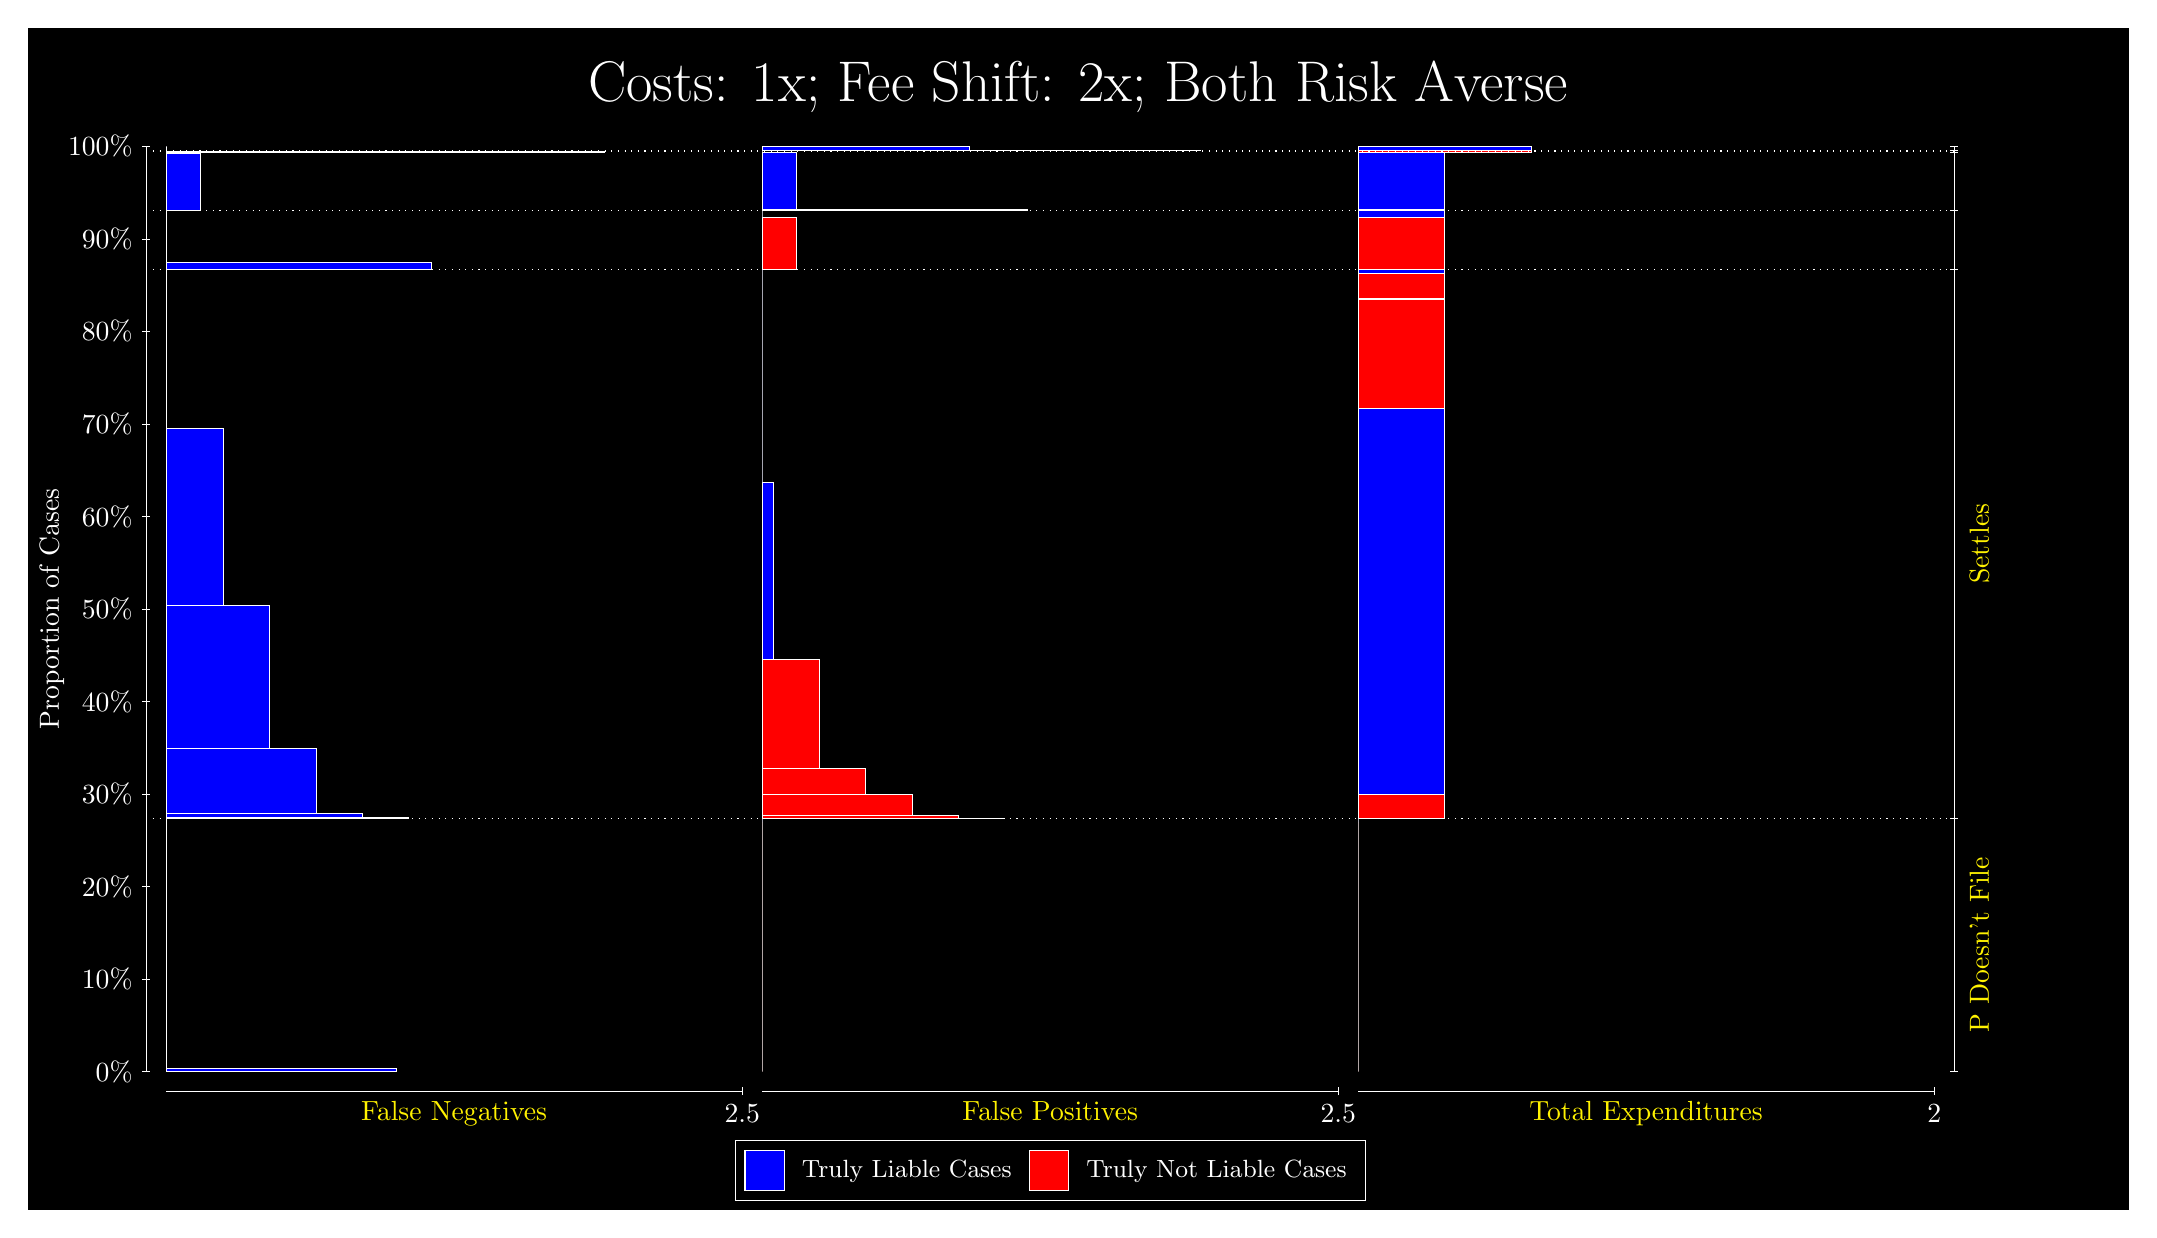
\begin{tikzpicture}
\draw[fill=black] (0,0) rectangle (26.667,15);
\draw[text=white] (0,13.5) rectangle (26.667,15) node[midway] {\huge Costs: 1x; Fee Shift: 2x; Both Risk Averse};
\draw[white, very thin] (1.5,1.75) -- (1.5,13.5);
\node[rotate=90, text=white, anchor=center] at (0.3, 7.625) {Proportion of Cases};
\draw[white, very thin] (1.45,1.75) -- (1.55,1.75);
\node[text=white, anchor=east] at (1.45, 1.75) {0\%};
\draw[white, very thin] (1.45,2.925) -- (1.55,2.925);
\node[text=white, anchor=east] at (1.45, 2.925) {10\%};
\draw[white, very thin] (1.45,4.1) -- (1.55,4.1);
\node[text=white, anchor=east] at (1.45, 4.1) {20\%};
\draw[white, very thin] (1.45,5.275) -- (1.55,5.275);
\node[text=white, anchor=east] at (1.45, 5.275) {30\%};
\draw[white, very thin] (1.45,6.45) -- (1.55,6.45);
\node[text=white, anchor=east] at (1.45, 6.45) {40\%};
\draw[white, very thin] (1.45,7.625) -- (1.55,7.625);
\node[text=white, anchor=east] at (1.45, 7.625) {50\%};
\draw[white, very thin] (1.45,8.8) -- (1.55,8.8);
\node[text=white, anchor=east] at (1.45, 8.8) {60\%};
\draw[white, very thin] (1.45,9.975) -- (1.55,9.975);
\node[text=white, anchor=east] at (1.45, 9.975) {70\%};
\draw[white, very thin] (1.45,11.15) -- (1.55,11.15);
\node[text=white, anchor=east] at (1.45, 11.15) {80\%};
\draw[white, very thin] (1.45,12.325) -- (1.55,12.325);
\node[text=white, anchor=east] at (1.45, 12.325) {90\%};
\draw[white, very thin] (1.45,13.5) -- (1.55,13.5);
\node[text=white, anchor=east] at (1.45, 13.5) {100\%};

\draw[white, very thin] (24.457,1.75) -- (24.457,13.5);
\draw[white, very thin] (24.407,1.75) -- (24.507,1.75);
\node[anchor=west] at (24.407, 1.75) {};
\draw[white, very thin] (24.407,4.9655) -- (24.507,4.9655);
\node[anchor=west] at (24.407, 4.9655) {};
\draw[white, very thin] (24.407,11.94) -- (24.507,11.94);
\node[anchor=west] at (24.407, 11.94) {};
\draw[white, very thin] (24.407,12.686) -- (24.507,12.686);
\node[anchor=west] at (24.407, 12.686) {};
\draw[white, very thin] (24.407,13.429) -- (24.507,13.429);
\node[anchor=west] at (24.407, 13.429) {};
\draw[white, very thin] (24.407,13.452) -- (24.507,13.452);
\node[anchor=west] at (24.407, 13.452) {};
\draw[white, very thin] (24.407,13.5) -- (24.507,13.5);
\node[anchor=west] at (24.407, 13.5) {};

\draw[white, very thin, fill=blue] (1.75,1.75) rectangle (4.6775,1.7972);
\draw[white, very thin, fill=red] (1.75,1.7972) rectangle (1.75,4.9655);
\draw[white, very thin, fill=blue] (1.75,4.9655) rectangle (4.8239,4.9784);
\draw[white, very thin, fill=blue] (1.75,4.9784) rectangle (4.2384,5.0279);
\draw[white, very thin, fill=blue] (1.75,5.0279) rectangle (3.6529,5.8533);
\draw[white, very thin, fill=blue] (1.75,5.8533) rectangle (3.0674,7.6721);
\draw[white, very thin, fill=blue] (1.75,7.6721) rectangle (2.4819,9.9206);
\draw[white, very thin, fill=red] (1.75,9.9206) rectangle (1.75,11.94);
\draw[white, very thin, fill=blue] (1.75,11.94) rectangle (5.1167,12.031);
\draw[white, very thin, fill=red] (1.75,12.031) rectangle (1.75,12.686);
\draw[white, very thin, fill=blue] (1.75,12.686) rectangle (2.1891,13.416);
\draw[white, very thin, fill=red] (1.75,13.416) rectangle (1.75,13.429);
\draw[white, very thin, fill=blue] (1.75,13.429) rectangle (7.3123,13.436);
\draw[white, very thin, fill=red] (1.75,13.436) rectangle (1.75,13.452);
\draw[white, very thin, fill=red] (1.75,13.452) rectangle (1.75,13.456);
\draw[white, very thin, fill=blue] (1.75,13.456) rectangle (1.75,13.5);
\draw[white, very thin, fill=red] (9.3189,1.75) rectangle (9.3189,4.9183);
\draw[white, very thin, fill=blue] (9.3189,4.9183) rectangle (9.3189,4.9655);
\draw[white, very thin, fill=red] (9.3189,4.9655) rectangle (12.393,4.9695);
\draw[white, very thin, fill=red] (9.3189,4.9695) rectangle (11.807,5.0107);
\draw[white, very thin, fill=red] (9.3189,5.0107) rectangle (11.222,5.2767);
\draw[white, very thin, fill=red] (9.3189,5.2767) rectangle (10.636,5.5959);
\draw[white, very thin, fill=red] (9.3189,5.5959) rectangle (10.051,6.9846);
\draw[white, very thin, fill=blue] (9.3189,6.9846) rectangle (9.4652,9.2331);
\draw[white, very thin, fill=blue] (9.3189,9.2331) rectangle (9.3189,11.94);
\draw[white, very thin, fill=red] (9.3189,11.94) rectangle (9.758,12.594);
\draw[white, very thin, fill=blue] (9.3189,12.594) rectangle (9.3189,12.686);
\draw[white, very thin, fill=red] (9.3189,12.686) rectangle (12.686,12.699);
\draw[white, very thin, fill=blue] (9.3189,12.699) rectangle (9.758,13.429);
\draw[white, very thin, fill=red] (9.3189,13.429) rectangle (9.3189,13.445);
\draw[white, very thin, fill=blue] (9.3189,13.445) rectangle (9.3189,13.452);
\draw[white, very thin, fill=red] (9.3189,13.452) rectangle (14.881,13.456);
\draw[white, very thin, fill=blue] (9.3189,13.456) rectangle (11.954,13.5);
\draw[white, very thin, fill=red] (16.888,1.75) rectangle (16.888,4.9183);
\draw[white, very thin, fill=blue] (16.888,4.9183) rectangle (16.888,4.9655);
\draw[white, very thin, fill=red] (16.888,4.9655) rectangle (17.986,5.2767);
\draw[white, very thin, fill=blue] (16.888,5.2767) rectangle (17.986,10.169);
\draw[white, very thin, fill=red] (16.888,10.169) rectangle (17.986,11.558);
\draw[white, very thin, fill=blue] (16.888,11.558) rectangle (17.986,11.571);
\draw[white, very thin, fill=red] (16.888,11.571) rectangle (17.986,11.89);
\draw[white, very thin, fill=blue] (16.888,11.89) rectangle (17.986,11.94);
\draw[white, very thin, fill=red] (16.888,11.94) rectangle (17.986,12.594);
\draw[white, very thin, fill=blue] (16.888,12.594) rectangle (17.986,12.686);
\draw[white, very thin, fill=red] (16.888,12.686) rectangle (17.986,12.699);
\draw[white, very thin, fill=blue] (16.888,12.699) rectangle (17.986,13.429);
\draw[white, very thin, fill=red] (16.888,13.429) rectangle (19.083,13.445);
\draw[white, very thin, fill=blue] (16.888,13.445) rectangle (19.083,13.452);
\draw[white, very thin, fill=red] (16.888,13.452) rectangle (19.083,13.456);
\draw[white, very thin, fill=blue] (16.888,13.456) rectangle (19.083,13.5);
\draw[white, dotted] (1.5,4.9655) -- (24.457,4.9655);
\draw[white, dotted] (1.5,11.94) -- (24.457,11.94);
\draw[white, dotted] (1.5,12.686) -- (24.457,12.686);
\draw[white, dotted] (1.5,13.429) -- (24.457,13.429);
\draw[white, dotted] (1.5,13.452) -- (24.457,13.452);
\draw[white, very thin] (1.75,1.5) -- (9.0689,1.5);
\node[text=yellow, anchor=north] at (5.4094, 1.5) {False Negatives};
\draw[white, very thin] (9.0689,1.45) -- (9.0689,1.55);
\node[text=white, anchor=north] at (9.0689, 1.45) {2.5};

\draw[white, very thin] (9.3189,1.5) -- (16.638,1.5);
\node[text=yellow, anchor=north] at (12.978, 1.5) {False Positives};
\draw[white, very thin] (16.638,1.45) -- (16.638,1.55);
\node[text=white, anchor=north] at (16.638, 1.45) {2.5};

\draw[white, very thin] (16.888,1.5) -- (24.207,1.5);
\node[text=yellow, anchor=north] at (20.547, 1.5) {Total Expenditures};
\draw[white, very thin] (24.207,1.45) -- (24.207,1.55);
\node[text=white, anchor=north] at (24.207, 1.45) {2};

\node[text=yellow, centered, rotate=90] at (24.777, 3.3577) {P Doesn't File};
\node[text=yellow, centered, rotate=90] at (24.777, 8.4526) {Settles};





\draw (12.978300999999998,1.5) node[draw=none] (baseCoordinate) {};
\begin{scope}[align=center]
        \matrix[scale=0.5, draw=white, below=0.5cm of baseCoordinate, nodes={draw}, column sep=0.1cm]{
            \node[rectangle, draw, minimum width=0.5cm, minimum height=0.5cm, fill=blue] {}; &
            \node[draw=none, font=\small, text=white] (B) {Truly Liable Cases}; &
            \node[rectangle, draw, minimum width=0.5cm, minimum height=0.5cm, fill=red] {}; &
            \node[draw=none, font=\small, text=white] (B) {Truly Not Liable Cases}; \\
            };
\end{scope}

\end{tikzpicture}
\end{document}